
\begin{figure}[H]
  {
    \setlength{\tabcolsep}{3.0pt}
    \setlength\cmidrulewidth{\heavyrulewidth} % Make cmidrule = 
    \begin{adjustbox}{height=5cm,center}
      \footnotesize
      \begin{tabular}{ll}

        \makecell[l]{
\icode{.BYTE \$00,\$00,\$01,\$01}\\
\icode{.BYTE \$00,\$FF,\$FE,\$FD}
} & \makecell[l]{
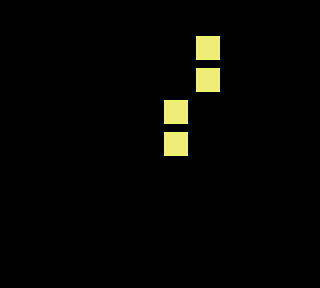
\includegraphics[width=1.3cm]{src/patterns/pixels/pixel_pattern13_0.png}%
} \\
        \midrule

        \makecell[l]{
\icode{.BYTE \$00,\$FF,\$FF,\$FE}\\
\icode{.BYTE \$00,\$01,\$02,\$03}
} & \makecell[l]{
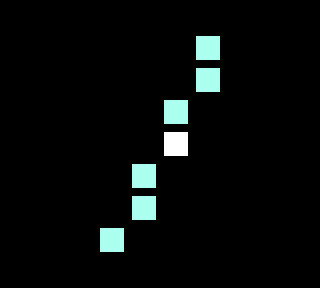
\includegraphics[width=1.3cm]{src/patterns/pixels/pixel_pattern13_1.png}%
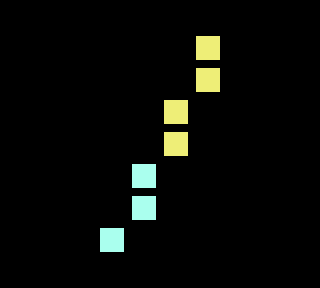
\includegraphics[width=1.3cm]{src/patterns/pixels/pixel_pattern13_2.png}%
} \\
        \midrule

        \makecell[l]{
\icode{.BYTE \$00,\$FD,\$FC,\$FB}\\
\icode{.BYTE \$00,\$04,\$04,\$03}
} & \makecell[l]{
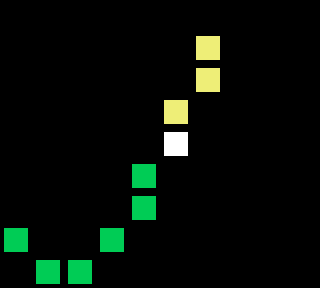
\includegraphics[width=1.3cm]{src/patterns/pixels/pixel_pattern13_3.png}%
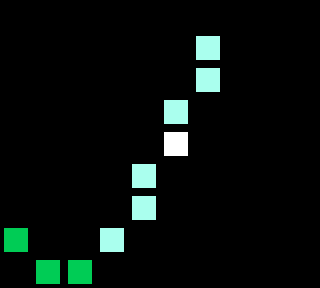
\includegraphics[width=1.3cm]{src/patterns/pixels/pixel_pattern13_4.png}%
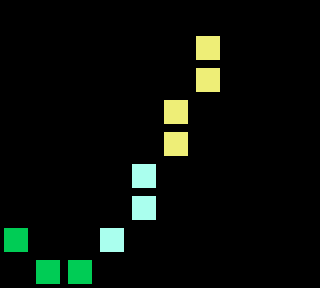
\includegraphics[width=1.3cm]{src/patterns/pixels/pixel_pattern13_5.png}%
} \\
        \midrule

        \makecell[l]{
\icode{.BYTE \$00,\$FD,\$FE,\$FF}\\
\icode{.BYTE \$00,\$FC,\$FC,\$FC}
} & \makecell[l]{
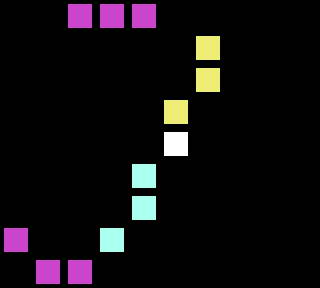
\includegraphics[width=1.3cm]{src/patterns/pixels/pixel_pattern13_6.png}%
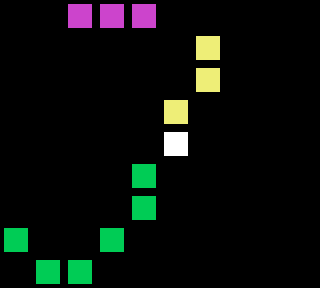
\includegraphics[width=1.3cm]{src/patterns/pixels/pixel_pattern13_7.png}%
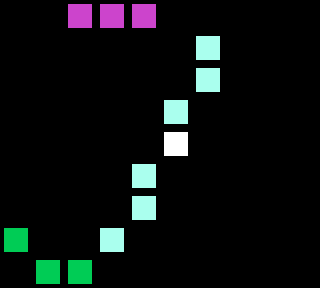
\includegraphics[width=1.3cm]{src/patterns/pixels/pixel_pattern13_8.png}%
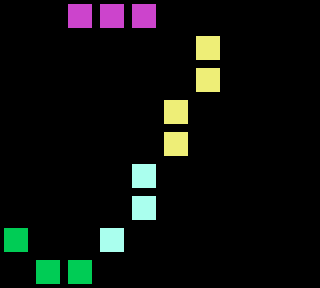
\includegraphics[width=1.3cm]{src/patterns/pixels/pixel_pattern13_9.png}%
} \\
        \midrule

        \makecell[l]{
\icode{.BYTE \$00,\$00,\$01,\$02}\\
\icode{.BYTE \$00,\$FC,\$FC,\$FC}
} & \makecell[l]{
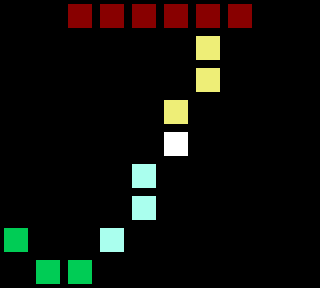
\includegraphics[width=1.3cm]{src/patterns/pixels/pixel_pattern13_10.png}%
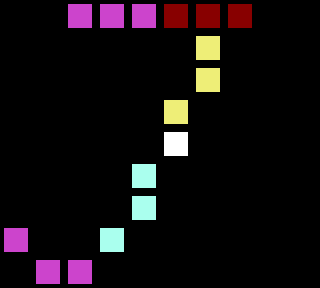
\includegraphics[width=1.3cm]{src/patterns/pixels/pixel_pattern13_11.png}%
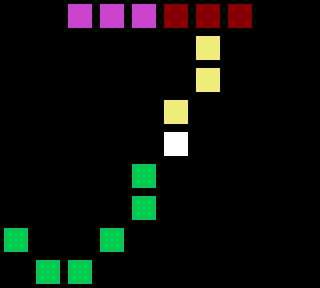
\includegraphics[width=1.3cm]{src/patterns/pixels/pixel_pattern13_12.png}%
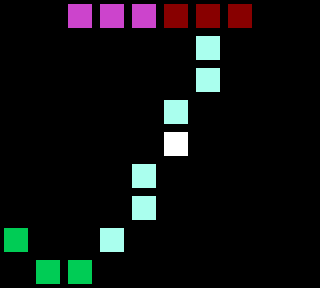
\includegraphics[width=1.3cm]{src/patterns/pixels/pixel_pattern13_13.png}%
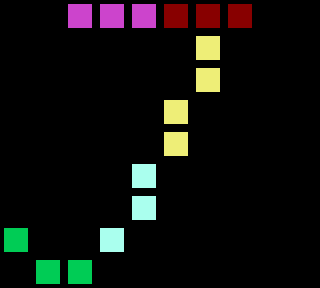
\includegraphics[width=1.3cm]{src/patterns/pixels/pixel_pattern13_14.png}%
} \\
        \midrule

        \makecell[l]{
\icode{.BYTE \$00,\$03,\$04}\\
\icode{.BYTE \$00,\$FC,\$FC}
} & \makecell[l]{
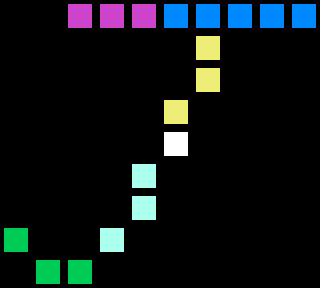
\includegraphics[width=1.3cm]{src/patterns/pixels/pixel_pattern13_15.png}%
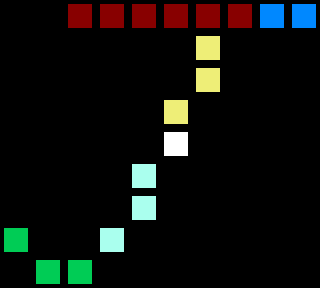
\includegraphics[width=1.3cm]{src/patterns/pixels/pixel_pattern13_16.png}%
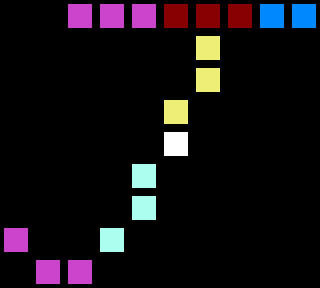
\includegraphics[width=1.3cm]{src/patterns/pixels/pixel_pattern13_17.png}%
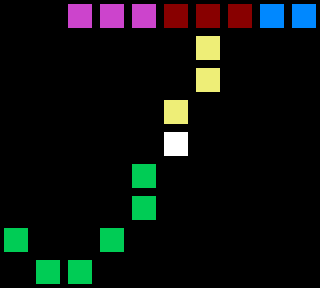
\includegraphics[width=1.3cm]{src/patterns/pixels/pixel_pattern13_18.png}%
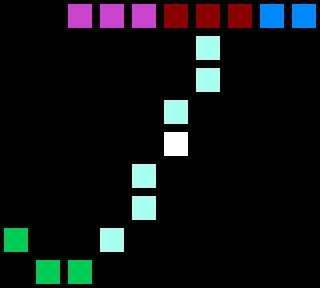
\includegraphics[width=1.3cm]{src/patterns/pixels/pixel_pattern13_19.png}%
} \\
        \midrule

        \makecell[l]{
\icode{.BYTE \$00}\\
\icode{.BYTE \$00}
} & \makecell[l]{
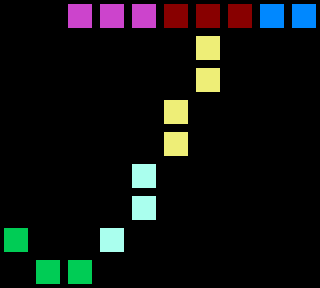
\includegraphics[width=1.3cm]{src/patterns/pixels/pixel_pattern13_20.png}%
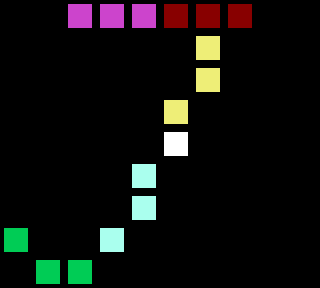
\includegraphics[width=1.3cm]{src/patterns/pixels/pixel_pattern13_21.png}%
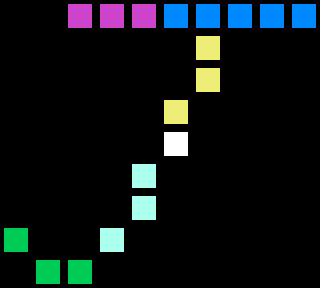
\includegraphics[width=1.3cm]{src/patterns/pixels/pixel_pattern13_22.png}%
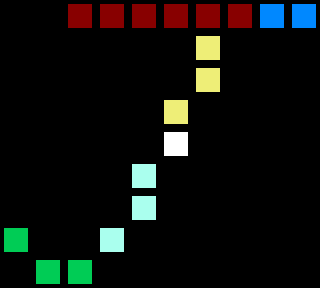
\includegraphics[width=1.3cm]{src/patterns/pixels/pixel_pattern13_23.png}%
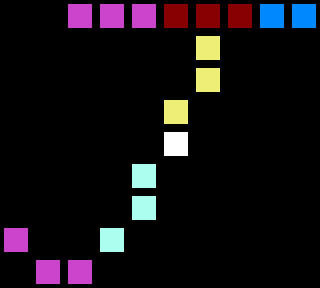
\includegraphics[width=1.3cm]{src/patterns/pixels/pixel_pattern13_24.png}%
} \\
        \midrule

      \end{tabular}
    \end{adjustbox}
  }\caption{The purpose of each of the oscillator values.}
\end{figure}
